\documentclass[aspectratio=169,xcolor=table]{beamer}
%aspcetratio >> 1610 169 149 54 43 32
%The themes:
% \usetheme[style=classic]{mharvellous}
%\usetheme[style=dark]{mharvellous}
%\usetheme[style=mracula]{mharvellous}
\usetheme[style=default]{mharvellous}
%*--------------------------------------------------
%\usepackage{helvet}
%*--------------------------------------------------
\usepackage{bibunits}  
%\setbeamertemplate{bibliography item}{[\theenumiv]}
\setbeamertemplate{bibliography item}{\insertbiblabel}
\defaultbibliography{bibliography}
%\defaultbibliographystyle{IEEEtran}
%\defaultbibliographystyle{amsalpha}
\defaultbibliographystyle{abntex2-alf}
%\bibliography{bibliography}
%\usepackage[backend=biber,style=alphabetic,citestyle=authoryear]{biblatex}
% \addbibresource{bibliography.bib}
%\usepackage{natbib}
\usepackage{bibentry}
%*--------------------------------------------------
\usepackage{lipsum}
\usepackage{epigraph}
\usepackage{graphicx}
\usepackage{multirow}
%\usepackage{enumitem}
\usepackage{array}
%\usepackage{multimedia}
\usepackage{media9}
%\usepackage{pdfpc-movie}
\usepackage{circledsteps}
\usepackage{listings}
\usepackage[normalem]{ulem}
%\usepackage{Sweave}
%\usepackage{xkeyval}
%\usepackage{palatino}
%\usepackage{pgfpages}
\usepackage{float}
%*--------------------------------------------------
\usepackage[timeinterval=1]{tdclock}
%\usepackage[font=Times,timeinterval=1, timeduration=200,resetatpages=all]{tdclock}
%\usepackage[font=Times,timeinterval=10, timeduration=2.0, timedeath=0, fillcolorwarningsecond=white!60!yellow,timewarningfirst=50,timewarningsecond=80,resetatpages=2]{tdclock}
%*--------------------------------------------------
\usepackage{url}
\usepackage{tabularx,booktabs}
\usepackage{threeparttable}
\usepackage[absolute, overlay]{textpos}
%*--------------------------------------------------
\usepackage{framed, color}
\usepackage[tikz]{bclogo}
\usepackage{spot}
\setspotlightcolor{red!50}
% %\setspotlightstyle{star, fill=red!50}
% %\setspotlightstyle{star points=7}
\usepackage{color,soul}
%\usepackage{xcolor}
\usepackage{tcolorbox}
\usepackage{xcolor}
\usepackage[export]{adjustbox}
\usepackage{verbatim}
\usetikzlibrary{trees,shapes,arrows}
\usepackage{fancyvrb}
\usepackage{float}
%*--------------------------------------------------
\usepackage{amsmath}
\usepackage{xfrac}
\usepackage{units}
\usepackage{ulem}
%*-------------------------------------------------------------------------------
%\newcolumntype{C}[1]{>{\centering\arraybackslash}m{#1}}
\newcolumntype{L}[1]{>{\raggedright\let\newline\\\arraybackslash\hspace{0pt}}m{#1}}
\newcolumntype{C}[1]{>{\centering\let\newline\\\arraybackslash\hspace{0pt}}m{#1}}
\newcolumntype{R}[1]{>{\raggedleft\let\newline\\\arraybackslash\hspace{0pt}}m{#1}}
%*-------------------------------------------------------------------------------
%\pgfpagesuselayout{2 on 1}[a4paper,border shrink=5mm]
%\setbeamertemplate{note page}[plain]
%\setbeameroption{show notes on second screen=bottom}
%*-------------------------------------------------------------------------------
\setbeameroption{hide notes}
%\setbeameroption{show only notes}
%\setbeameroption{show notes on second screen=right}
\setbeamertemplate{note page}{\pagecolor{yellow!5}\insertnote}
%*-------------------------------------------------------------------------------

%*-------------------------------------------------------------------------------
\title              {Manipuladores}
\subtitle           {Reunião semanal}
\author             {Juliana Santana}
\email              {juliana.maria@fbter.org.br}
\advisor            {Orientador: Marco A. dos Reis}
\institute          {Robótica e Sistemas Autônomos, Senai Cimatec}
\date               {Abril de 2022}
% \ulogo        		{Template/logosenaicimatecnegativo}
% \ulogof             {Template/logosenaicimatec2020}
% \ulogoo        		{Template/rosa-logo}
% \ulistelement    	{Template/bullet-white}

%*-------------------------------------------------------------------------------
\graphicspath{{Source/pictures/}}
%*-------------------------------------------------------------------------------
\totalNoSlidesDisabled % To turn off the total number of slides in the footer. Comment this if you want the total number of slides in the footer
%*-------------------------------------------------------------------------------
\begin{document}
%*----------- COVER -------------------------------------------------------------
 \begin{frame}[t,plain]
%*----------- sound--------------------------------
    \includemedia[
        %width=1ex,
        %height=1ex,
        %activate=pageopen, 
        activate=onclick,
        deactivate=onclick,
        %passcontext,
        transparent,
        addresource=./Source/sounds/hip-hop.mp3,
        flashvars={
                    source=./Source/sounds/hip-hop.mp3
                    %&autoPlay=true
                    &autoRewind=true
                    &Play=2s
                    &repeat=always
                    %&Loop=true
        }
    ]
    {}{VPlayer.swf}
%*----------- start-page--------------------------
    \titlepage
    %*----------- notes-------------------------------
    \note[item]{Notes can help you to remember important information. Turn on the notes option.}
\end{frame}
%-
%*----------- SECTIONS ----------------------------------------------------------
%*----------- SLIDE -------------------------------------------------------------
\begin{frame}[t]{A Álgebra Linear} 

 É uma área da matemática que que permite estudos matemáticos mais aprofundados e soluções em aplicações práticas em diversos campos da ciência e negócios.
 \nocite{baldin2011geometria}\nocite{boldrini1980algebra}\nocite{craig2012robotica}

 \vspace*{0.8cm}

\begin{figure}
    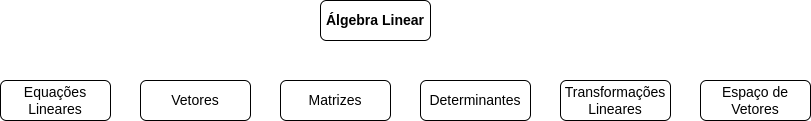
\includegraphics[width=\textwidth]{intro2.png}
\end{figure}
            
    \note[item]{Notes can help you to remember important information. Turn on the notes option.}
\end{frame}
%-

%*----------- SLIDE -------------------------------------------------------------
\begin{frame}[t]{Matriz e Vetores} 
    \begin{columns}
        \column{.01\textwidth}
        \column{.50\textwidth}
        \begin{itemize}
            \item Permitem escrever sistemas lineares de uma forma mais compacta
            \item E, utilizar operações com as matrizes para solucionar o sistema.
        \end{itemize}
        \column{.5\textwidth}
        \begin{figure}
            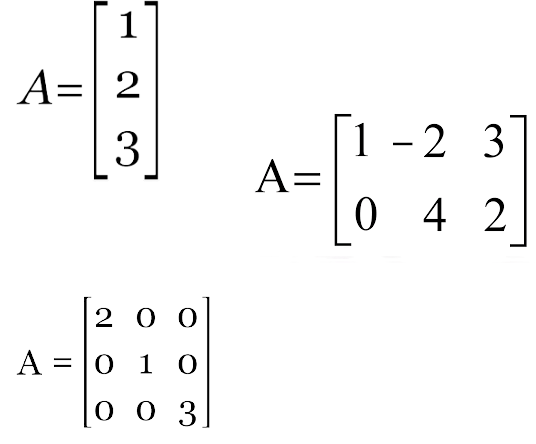
\includegraphics[width=0.8\textwidth]{matriz.png}
        \end{figure}
    \end{columns}
%*----------- notes
    \note[item]{Notes can help you to remember important information. Turn on the notes option.}
\end{frame}
%-
% %*----------- SLIDE -------------------------------------------------------------
\begin{frame}[c]{} 
    % \transdissolve[duration=0.5]
   
    \begin{center}
        \Wider{%
        \begin{shaded}
        \begin{center}
            \vspace*{0.3cm}
            \resizebox{!}{0.6cm}{%
                Walker
            }%
        \end{center}
        \end{shaded}
        }%
    \end{center}
       
%*----------- notes
    \note[item]{Notes can help you to remember important information. Turn on the notes option.}
\end{frame}
%
%*----------- SLIDE -------------------------------------------------------------
\begin{frame}[t]{Introdução} 
    Este projeto consiste em desenvolver um robô de pequeno porte que se desloca sobre dois pés. O robô deve ser capaz de se locomover e desviar de obstáculos em um determinado ambiente. Além disso, os \textbf{objetivos especifícos} são:
   
        \begin{columns}[c]
            \column{.6\textwidth}
                \begin{itemize}
                    \item Desenvolver algoritmos utilizando ROS;
                    \item Utilizar visão computacional;
                    \item Simular um robô no gazebo;
                    \item Desenvolver habilidades de gestão de projetos.
                \end{itemize}
            \column{.25\textwidth}
                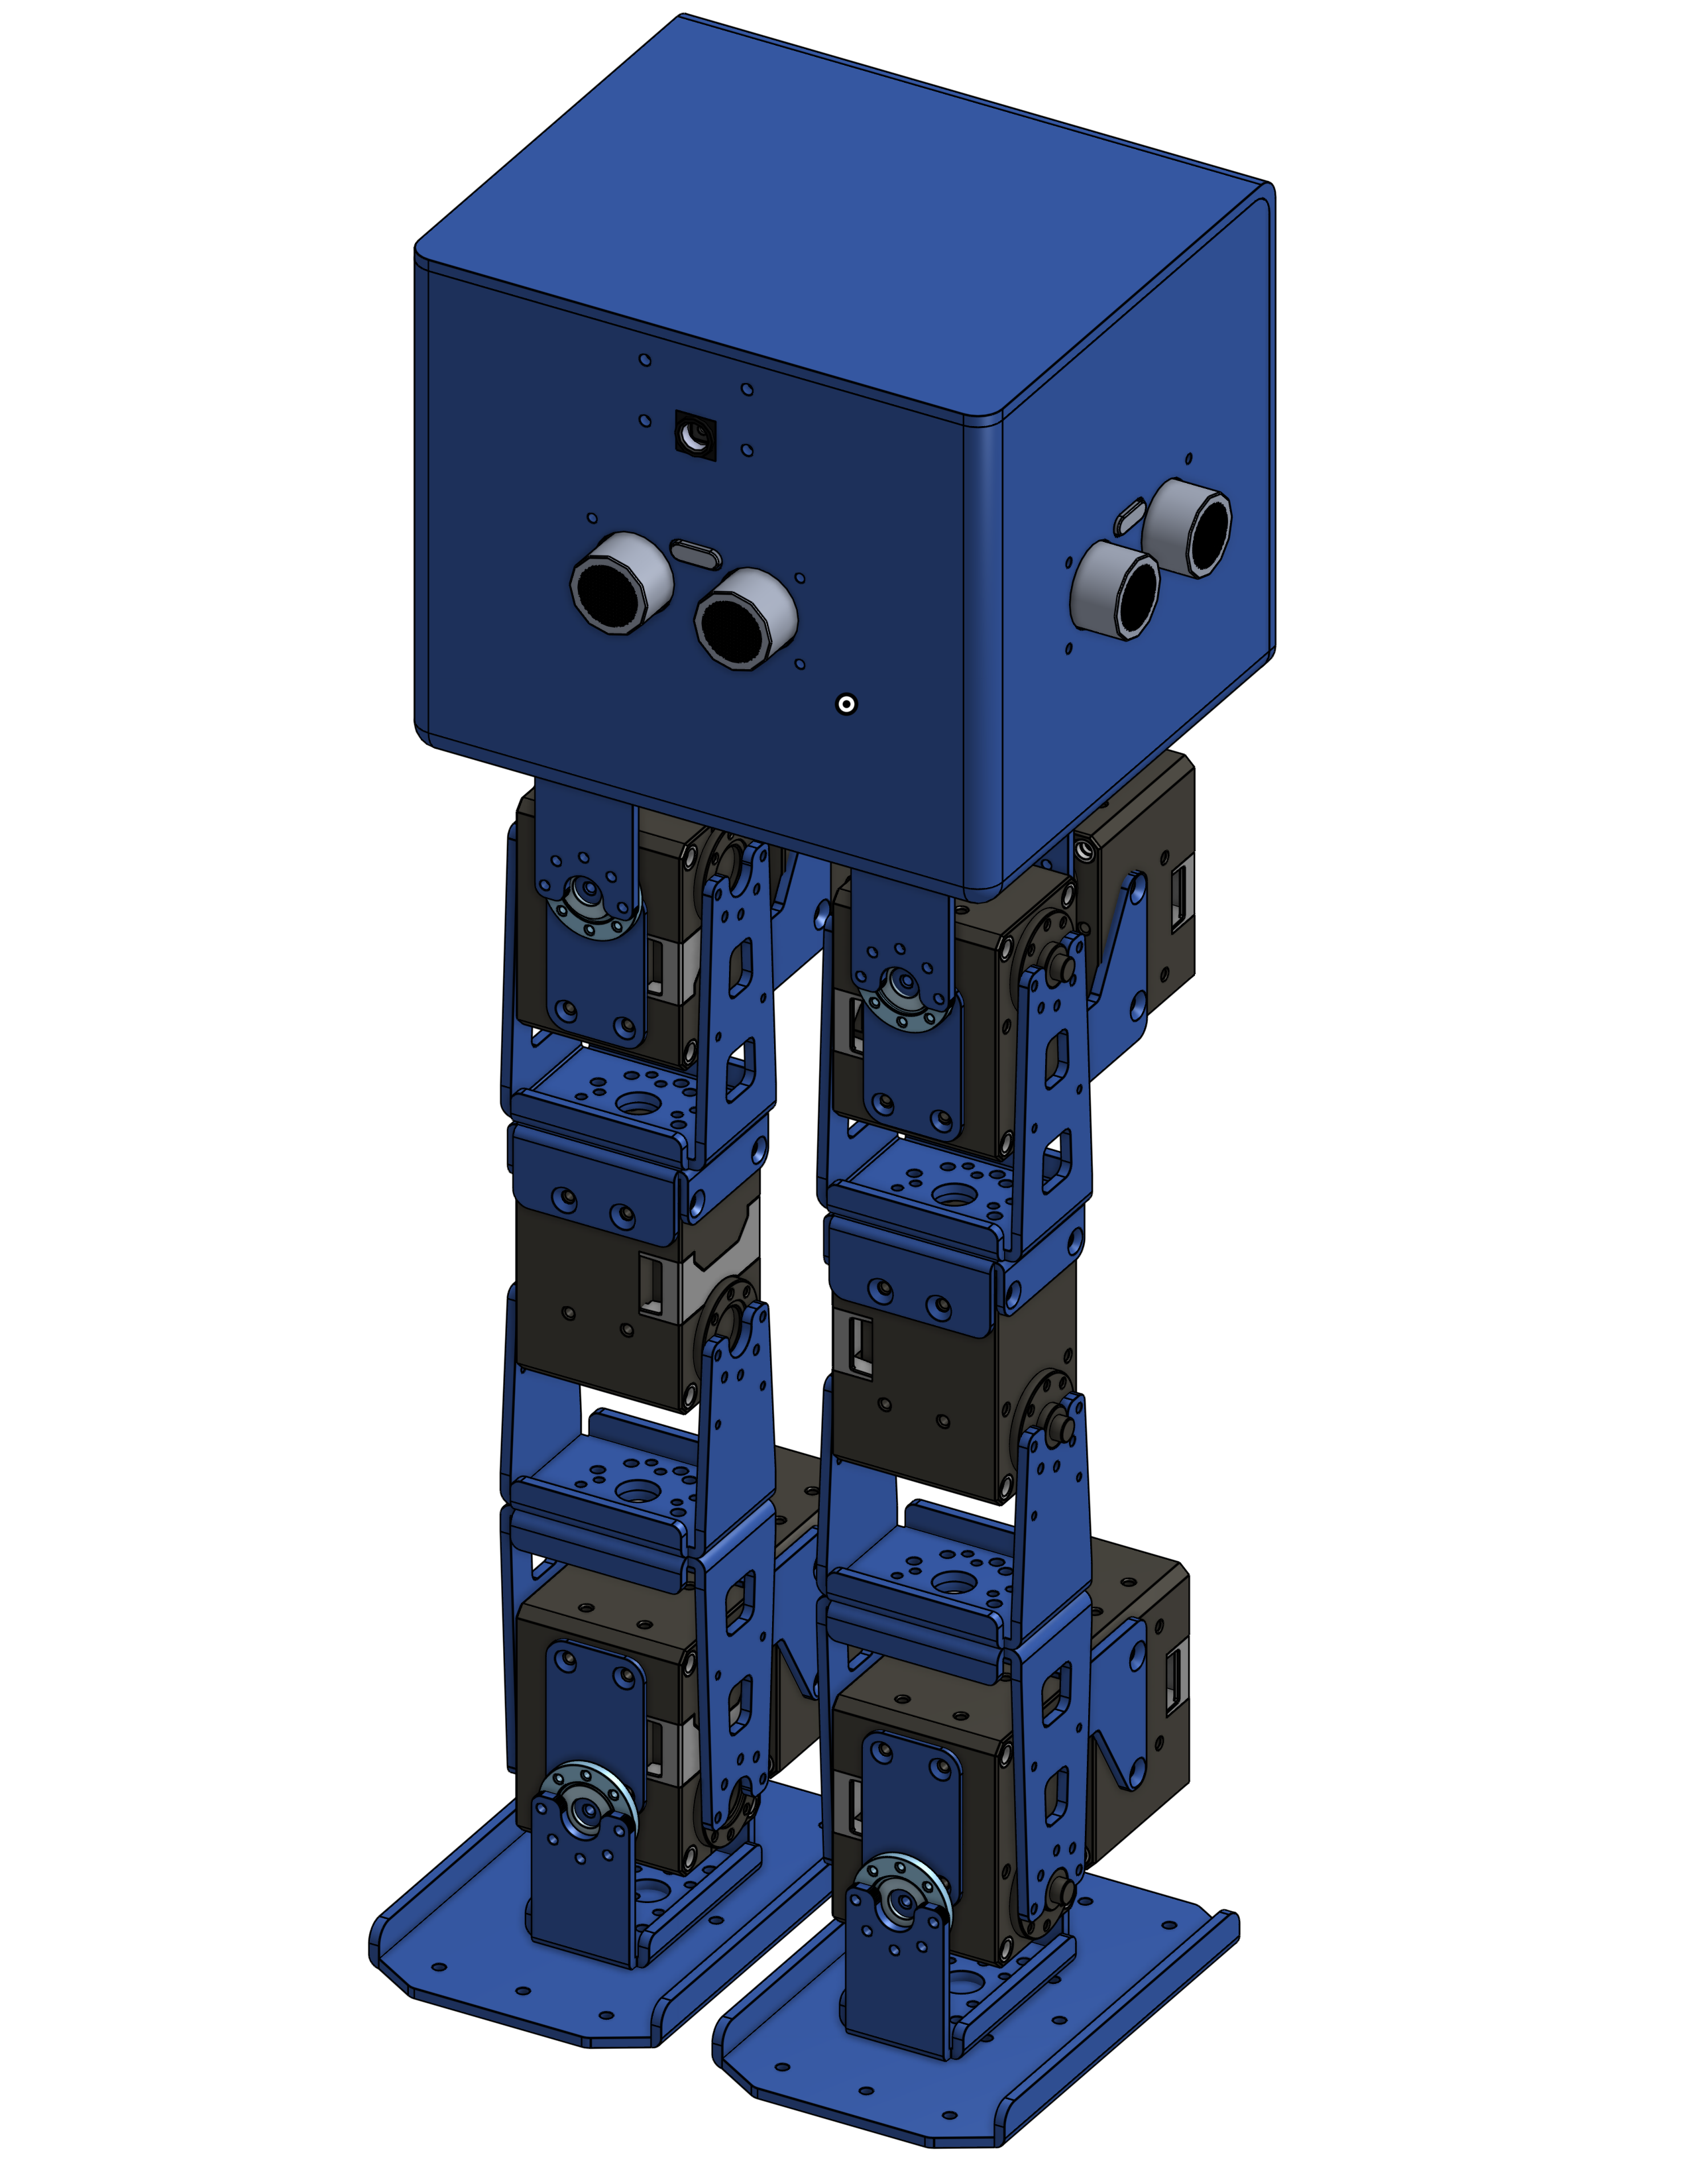
\includegraphics[width=1.1\textwidth]{walker3D}
        \end{columns}

\end{frame}
%-

%*----------- SLIDE -------------------------------------------------------------
\begin{frame}[t]{Missão do robô} 
    O Walker deve realizar uma missão, em um ambiente real, que consiste em:
    \newline
    \begin{columns}[c]
        \column{.6\textwidth}
            \begin{itemize}
                \item Navegar por um ambiente, de 
                forma autônoma;
                \item Reconhecer uma TAG;
                \item Encontrar um objeto (esfera) 
                em determinada região.
            \end{itemize}
        \column{.35\textwidth}
                \hspace{2cm}
\includegraphics[width=0.3
                \textwidth]{aruco}
                \newline
                
\includegraphics[width=0.3
                \textwidth]{esfera}
    \end{columns}
        
\end{frame}
%-


%*----------- SLIDE -------------------------------------------------------------
\begin{frame}[t]{Requisitos do Cliente} 
    \begin{columns}[c]
        \column{.6\textwidth}
            \begin{itemize}
                \item Operar em uma área de 2m x 1,5m;
                \item Possuir uma altura de aproximadamente 30 cm;
                \item Ser capaz de operar por, no mínimo, 20 min;
                \item Ser capaz de desviar de obstáculos.
            \end{itemize}
        \column{.35\textwidth}
            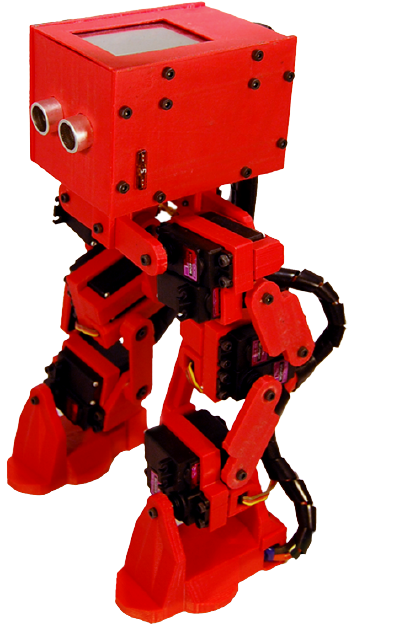
\includegraphics[width=0.7\textwidth]{biped}
    \end{columns}

\end{frame}
%-


%*----------- SLIDE -------------------------------------------------------------
\begin{frame}[t]{Requisitos técnicos} 
\begin{columns}
    \column{.0\textwidth}
    \column{.30\textwidth}
        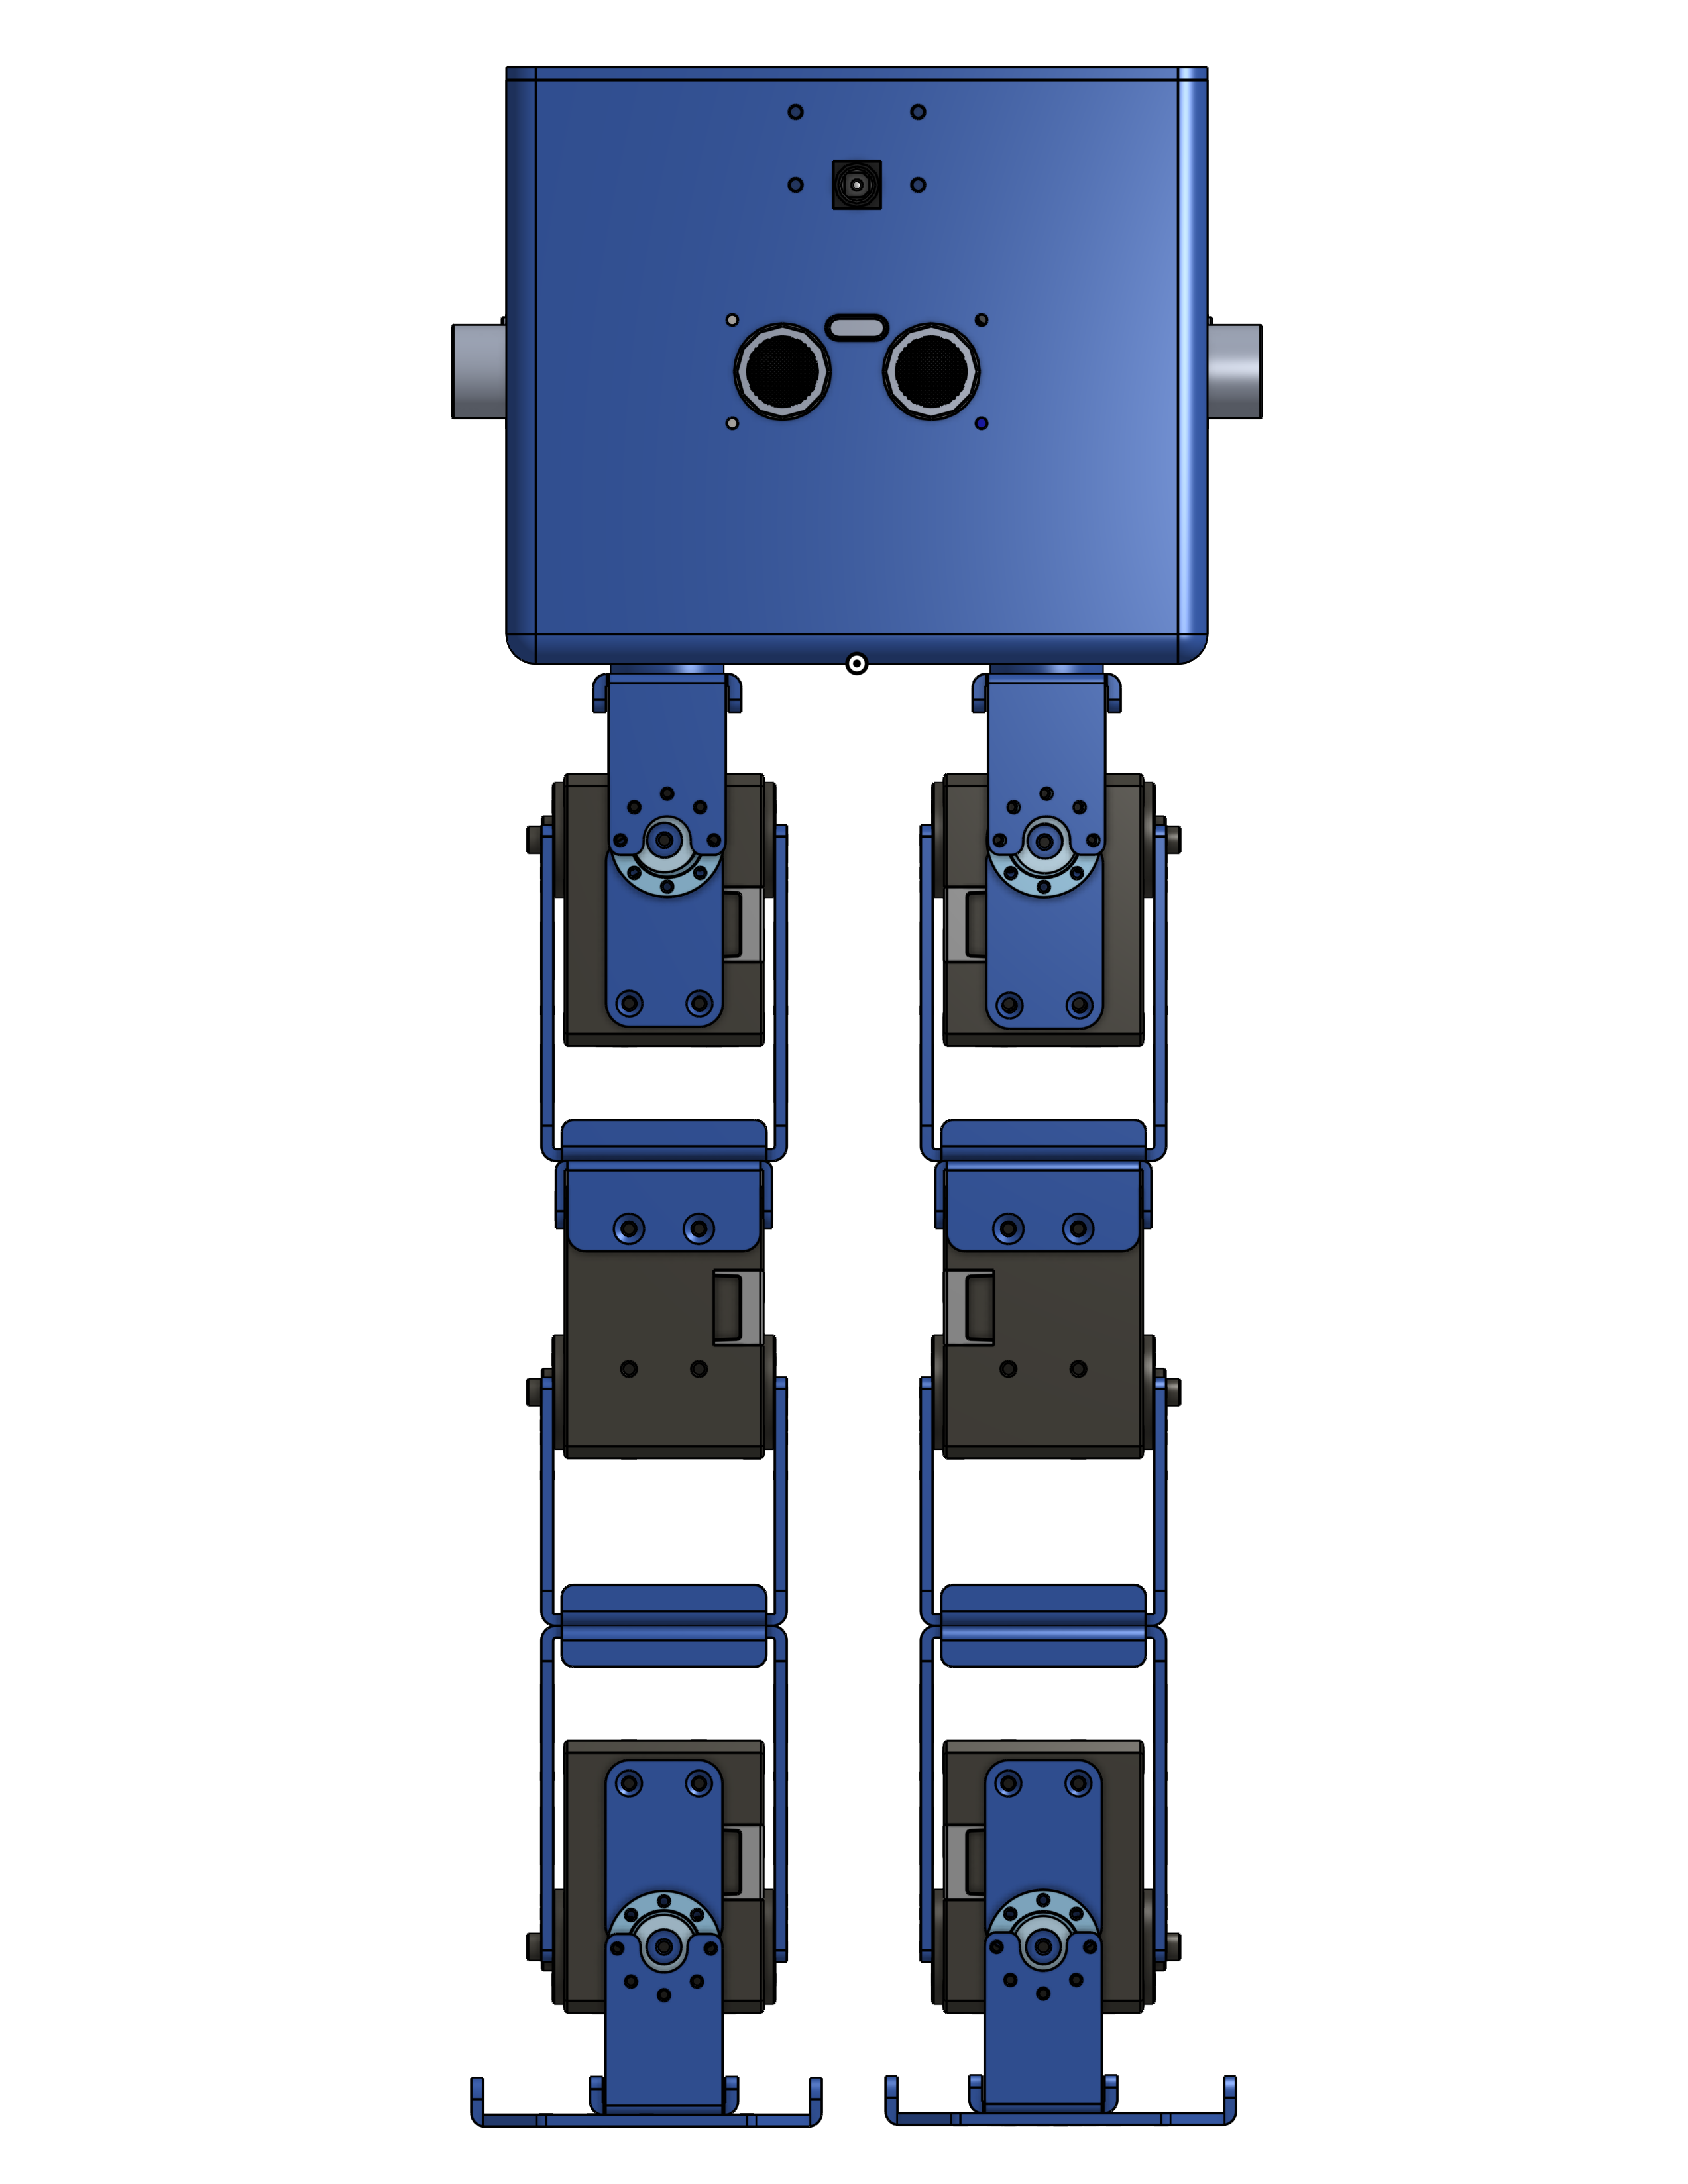
\includegraphics[width=\textwidth]{walker_3Dfrontal}
    \column{.7\textwidth}
        \begin{enumerate}
            \item Uso de servomotores com torque adequado ao deslocamento de uma caraga de massa 2kg
            \item Uso de sensor ativo para detecção de objetos a uma distância de 2,5m 
            \item Uso de câmera de espectro vísivel 
            \item ARM com 4GB de RAM
            \item ROS
            \item Ubuntu 20.04 + ROS Noetic
            \item Baterias Lithium de 10V a 14,8V
            \item Massa máxima de 2kg
        \end{enumerate}
\end{columns}

\end{frame}
%-


%*----------- SLIDE -------------------------------------------------------------
\begin{frame}[t]{Estrutura Analítica do Projeto} 
    \centering
    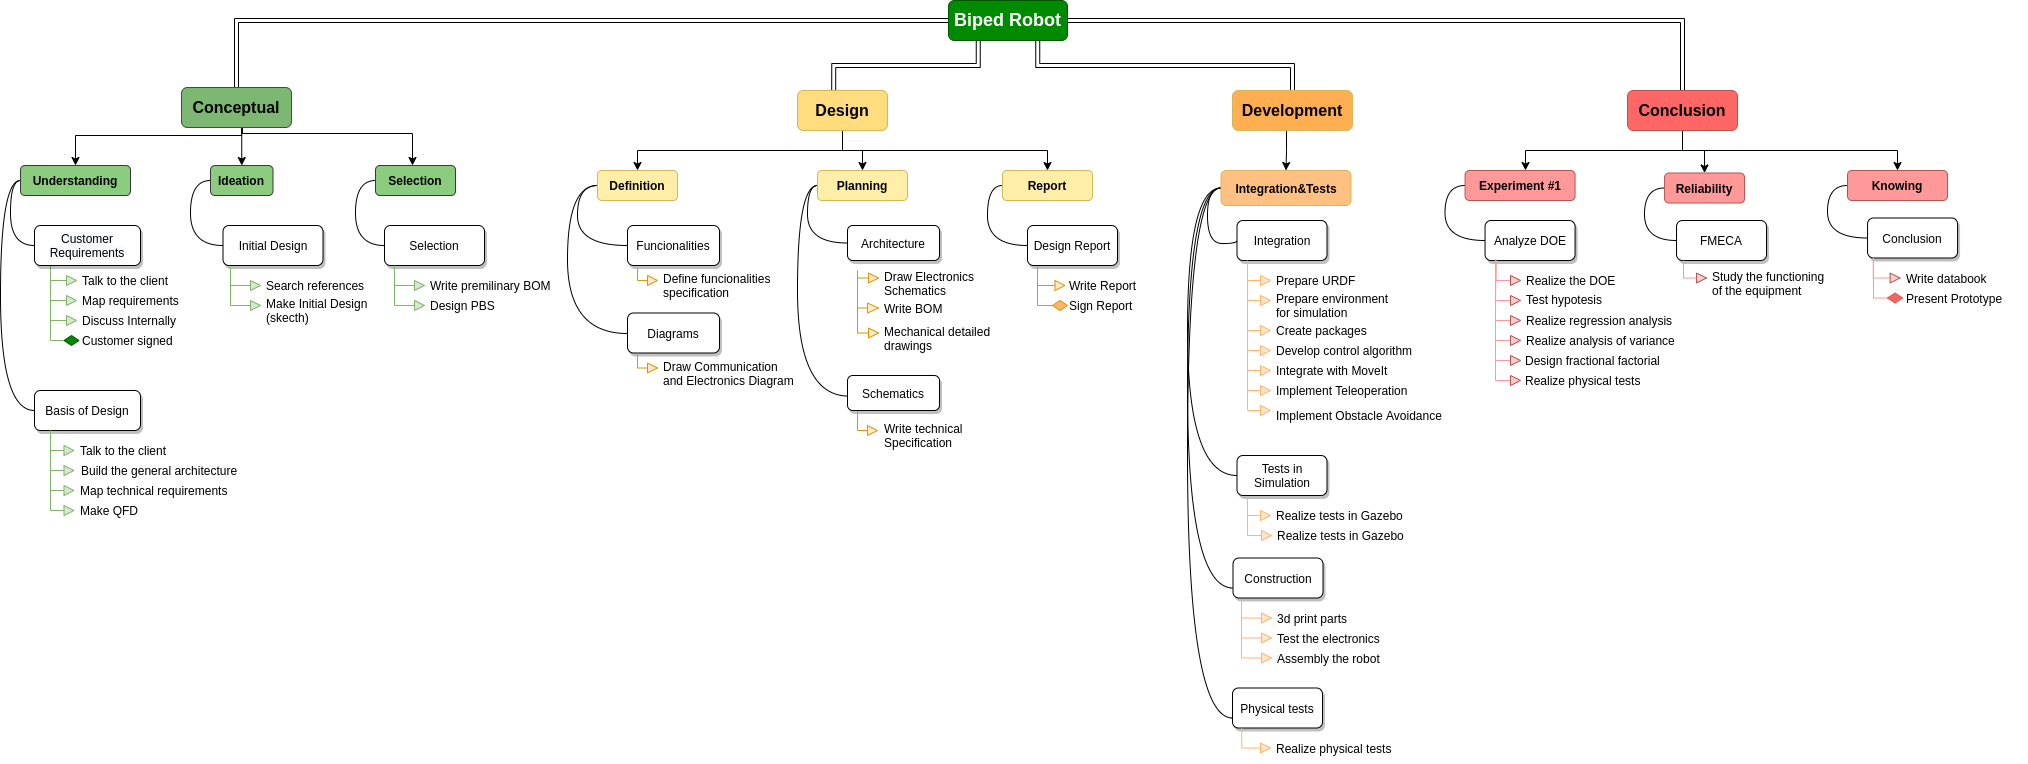
\includegraphics[width=\textwidth]{EAP}
        
\end{frame}
%-


%*----------- SLIDE -------------------------------------------------------------
\begin{frame}[t]{Cronograma} 
    \begin{columns}
        \column{.57\textwidth}
            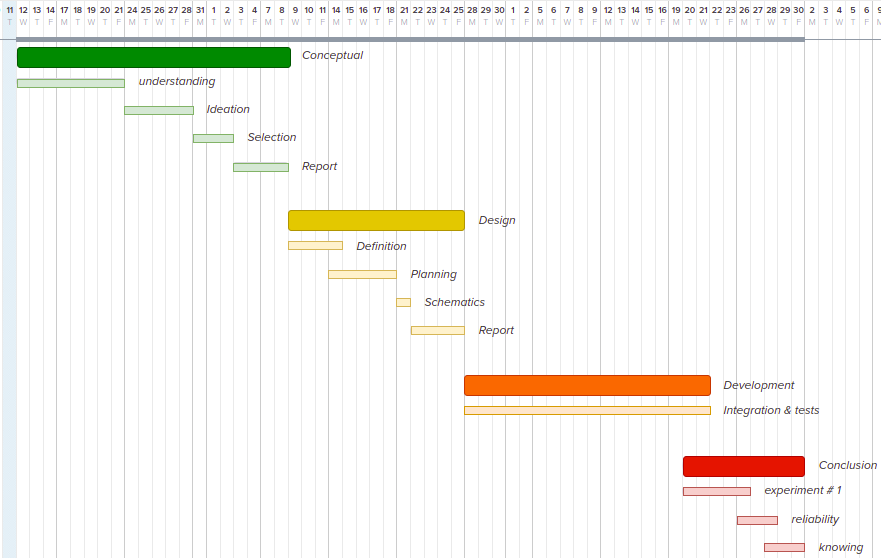
\includegraphics[width=1.1\textwidth]{cronograma_geral}
        \column{.41\textwidth}
            \begin{itemize}
                \item \textbf{Conceptual:} Semanas 0 a 4
                \item \textbf{Design:} Semanas 4 a 6
                \item \textbf{Development:} Semanas 6 a 10
                \item \textbf{Conclusion:} Semanas 10 a 11
            \end{itemize}
    \end{columns}
        
\end{frame}
%-


%*----------- SLIDE -------------------------------------------------------------
\begin{frame}[t]{Arquitetura Geral do Sistema} 

    \centering
    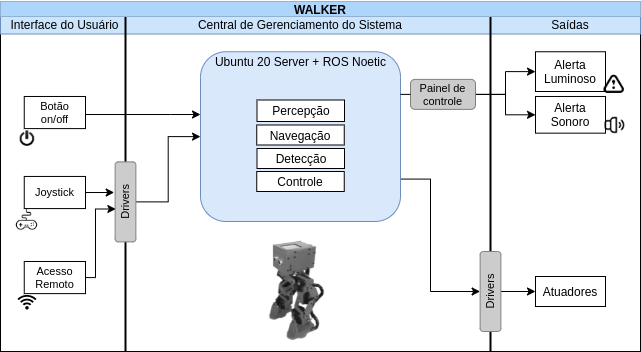
\includegraphics[width=.8\textwidth]{arquitetura_geral}

\end{frame}
%-


%*----------- SLIDE -------------------------------------------------------------
\begin{frame}[t]{Pesquisa por similares}
\begin{columns}
    \column{.35\textwidth}
        \centering    
            \newline \newline 
            \hspace{1.5cm}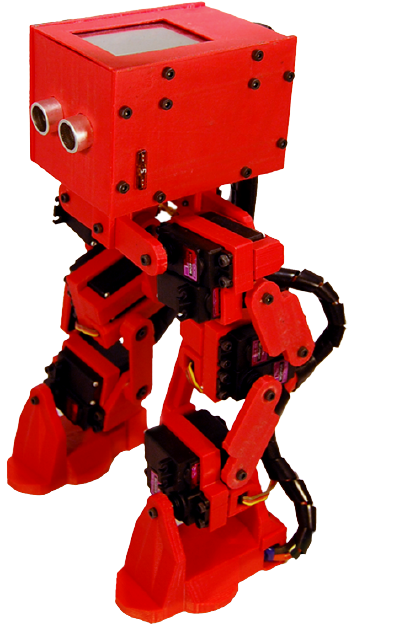
\includegraphics[width=.55\textwidth]{biped.png}
                \\ ROFI 
    \column{.35\textwidth}
        \centering
            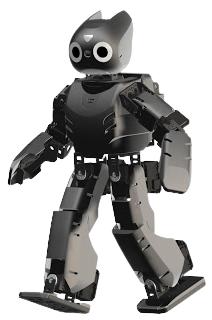
\includegraphics[width=.65\textwidth]{darwin.png}
            \\ Darwin-OP 
    \column{.35\textwidth}
        \centering
            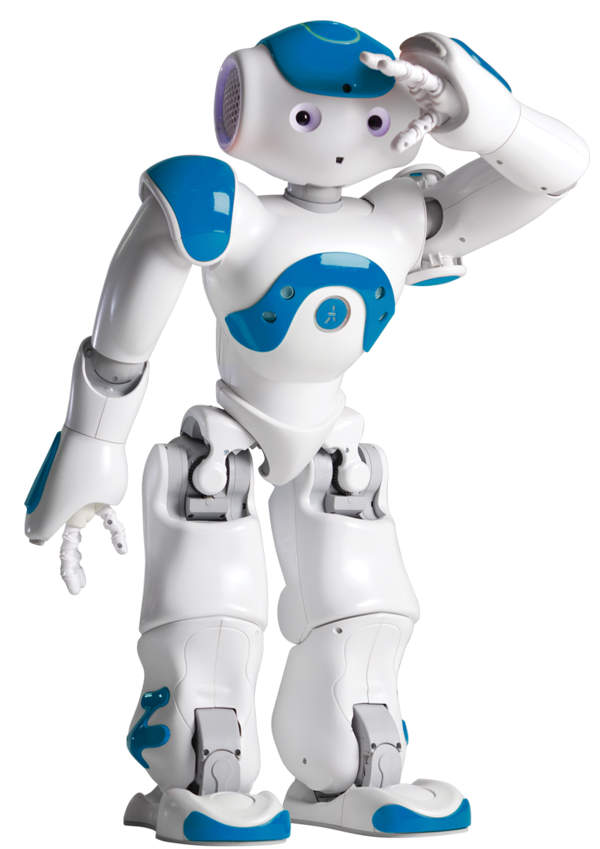
\includegraphics[width=.65\textwidth]{nao.png}
            \\ NAO
\end{columns}
\end{frame}
%-


%*----------- SLIDE -------------------------------------------------------------
\begin{frame}[t]{Product Breakdown Structure (PBS)} 
\centering
\vspace{1cm}
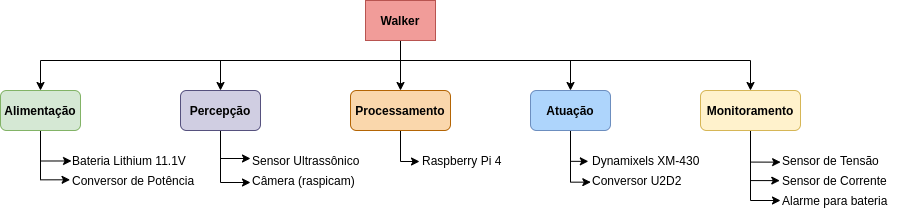
\includegraphics[width=\textwidth]{PBS_walker.png}
\end{frame}
%-


%*----------- SLIDE -------------------------------------------------------------
\begin{frame}[t]{Elaboração do QFD} 

    Com o objetivo de incorporar as necessidades do cliente ao projeto,
    \\ foi realizado o CFD (Desdobramento da Função Qualidade)
    \begin{columns}
        \column{.4\textwidth}
            \footnotesize
            \begin{itemize}
                \item \textbf{Técnicos x Técnicos} 
                \begin{itemize}
                    \footnotesize
                    \item Fortemente positivo  $\bullet$
                    \item Positivo $\circ$
                    \item Negativo $\ast$
                    \item Fortemente negativo $\diamondsuit$
                \end{itemize}
                \footnotesize
                \item \textbf{Cliente x Técnicos}
                \begin{itemize}
                    \footnotesize
                    \item Relações fortes $\bullet $
                    \item Relações médias $\circ $
                    \item Relações fracas $\bigtriangleup$
                \end{itemize}
            \end{itemize}
        \column{.56\textwidth}
            \vspace{-1.55cm}
            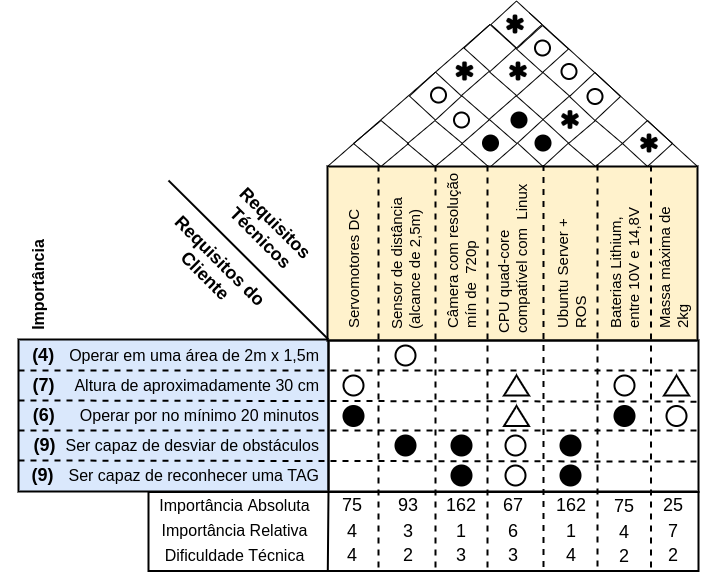
\includegraphics[width=\textwidth]{QFD}
    \end{columns}

\end{frame}


%*----------- SLIDE -------------------------------------------------------------
\begin{frame}[t]{Especificação de Funcionalidades} 
    \centering
    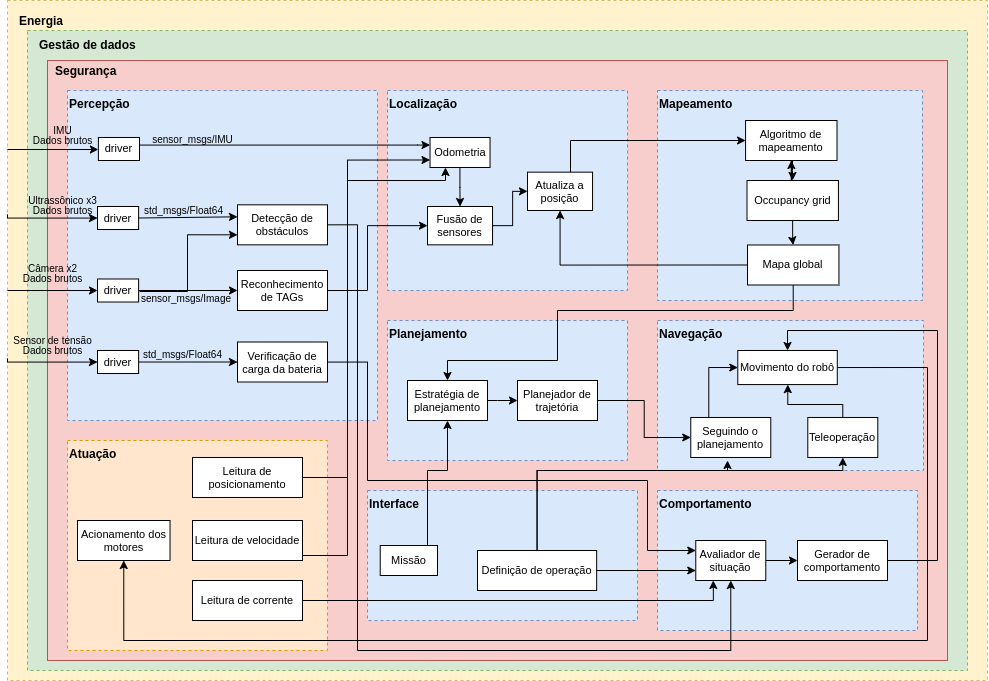
\includegraphics[width=.68\textwidth]{funcionalidades}

\end{frame}
%-


\begin{frame}[t]{Andamento do projeto} 
    \begin{columns}
        \column{.6\textwidth} 
            \centering \textbf{Realizado X Planejado: } x\%
            \begin{table}[]
                \begin{tabular}{@{}
                >{\columncolor[HTML]{C8D2EC}}l 
                >{\columncolor[HTML]{C8D2EC}}c @{}}
                \toprule
                \multicolumn{1}{c}{\cellcolor[HTML]{C8D2EC}{\color[HTML]{333333} \textbf{Biped Robot}}} & {\color[HTML]{333333} \textbf{36\%$\rightarrow$55\% }} \\ \midrule
                {\color[HTML]{333333} \textbf{Conceptual}}                                                       & {\color[HTML]{333333} \textbf{100\%$\rightarrow$100\%}} \\
                \textbf{Design}                                                                                  & \textbf{61\%$\rightarrow$96\%}                        \\
                \textbf{Development}                                                                             & \textbf{0\%$\rightarrow$9\%}                         \\
                {\color[HTML]{333333} \hspace{.2cm} Definition}                                                  & 0\%$\rightarrow$9\%                  \\
                \hspace{.2cm} Integration                                                                        & 0\%                                  \\
                \hspace{.2cm} Tests in Simulation                                                                & 0\%                                  \\
                \hspace{.2cm} Construction                                                                       & 0\%                                  \\
                \hspace{.2cm} Physical tests                                                                     & 0\%                                  \\
                \textbf{Conclusion}                                                                              & \textbf{0\%}                         \\ \bottomrule
                \end{tabular}
            \end{table}
        \column{.5\textwidth} 
            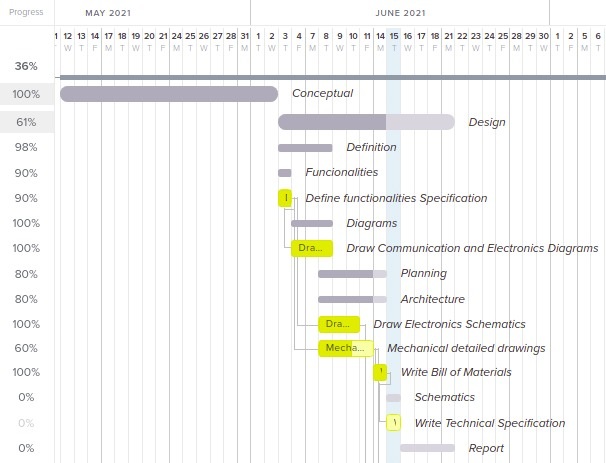
\includegraphics[width=1\textwidth]{andamento}
    \end{columns}
\end{frame}


%*----------- SLIDE -------------------------------------------------------------
\begin{frame}[t]{2 ciclo do QFD} 
    \begin{columns}
        \column{.4\textwidth}
        \footnotesize
        % \begin{itemize}
            \footnotesize
            % \item \textbf{Cliente x Técnicos}
            % \begin{itemize}
                %     \footnotesize
                %     \item Relações fortes $\bullet $
                %     \item Relações médias $\circ $
                %     \item Relações fracas $\bigtriangleup$
                % \end{itemize}
                \textbf{Targets} 
                \begin{itemize}
                    \footnotesize
                    \item Realizar a comunicação e a aquisição dos dados
                    \item Realizar a odometria e a atualização da posição
                    \item Realizar o mapeamento da área
                    \item Definir e planejar a trajetória
                    \item Elaborar os movimentos do roô
                    \item Definir a missão e o modo de operação
                    \item Avaliar as situações de alimentação e comportamento
                    \item Realizar a comunicação e aquisição de dados com os atuadores
                \end{itemize}
                % \end{itemize}
        \column{.4\textwidth}
            \newline
            \vspace{-0.55cm}
            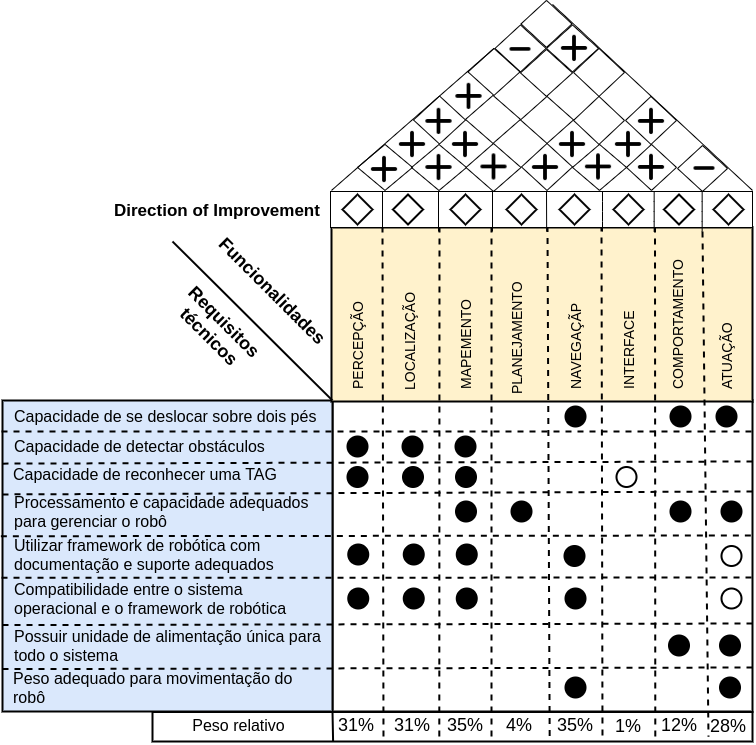
\includegraphics[width=1.2\textwidth]{2qfd}
    \end{columns}
    
\end{frame}
%-
%*----------- SLIDE -------------------------------------------------------------
\begin{frame}[t]{Shield PCB} 
    \begin{columns}
        \column{.5\textwidth}
        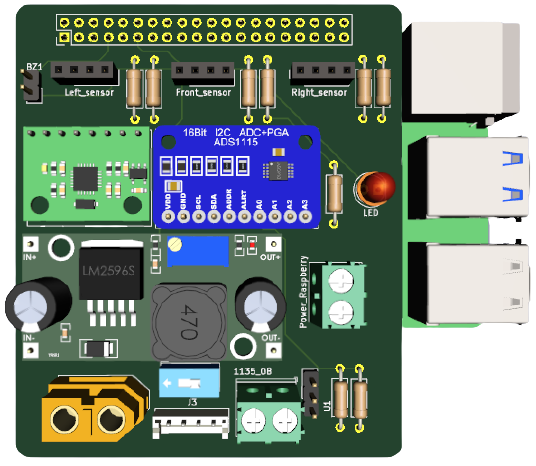
\includegraphics[width=\textwidth]{shield}

        \column{.5\textwidth}
        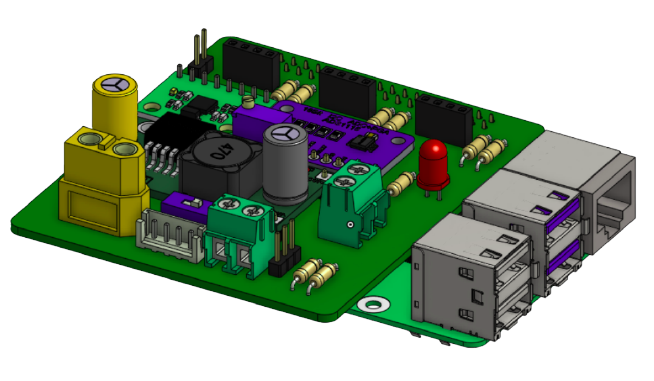
\includegraphics[width=1.1\textwidth]{shield_onshape.png}
        \vspace{-1cm}

    \end{columns}
\end{frame}
%-


%*----------- SLIDE -------------------------------------------------------------
\begin{frame}[t]{Desenhos Mecânicos} 
    \begin{columns}
        \column{.22\textwidth}
        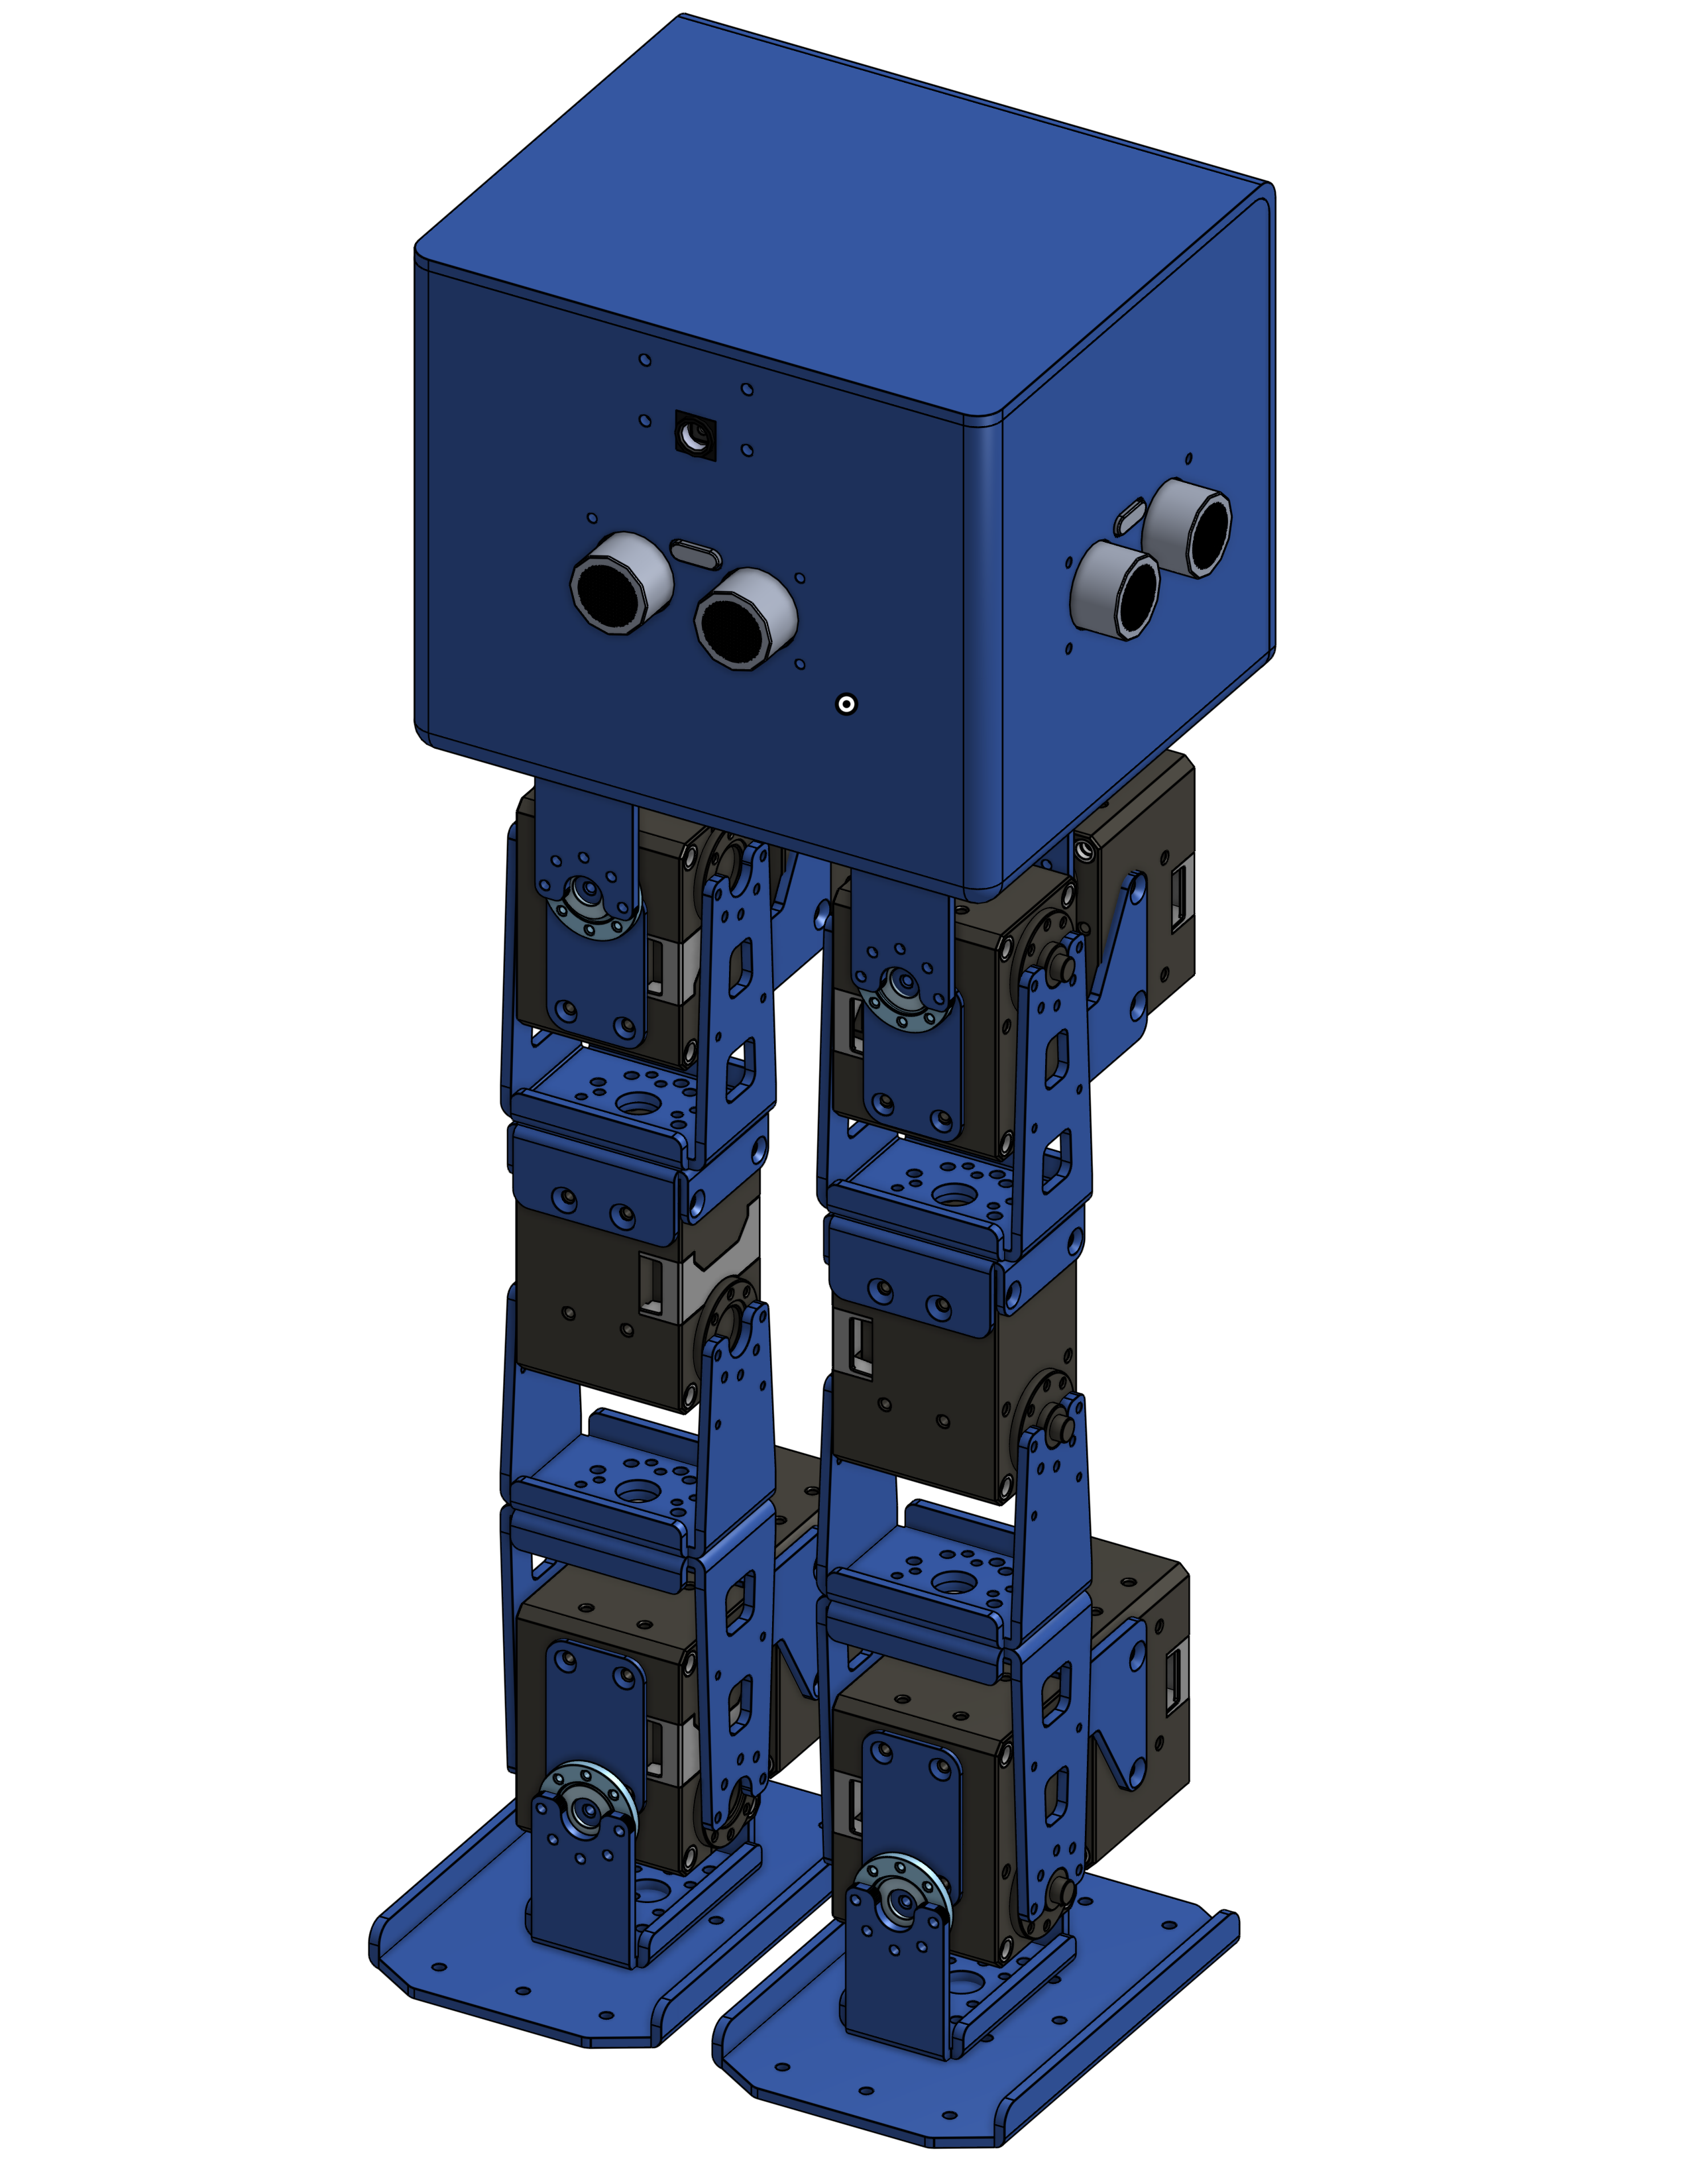
\includegraphics[width=\textwidth]{walker3D}

        \column{.22\textwidth}
        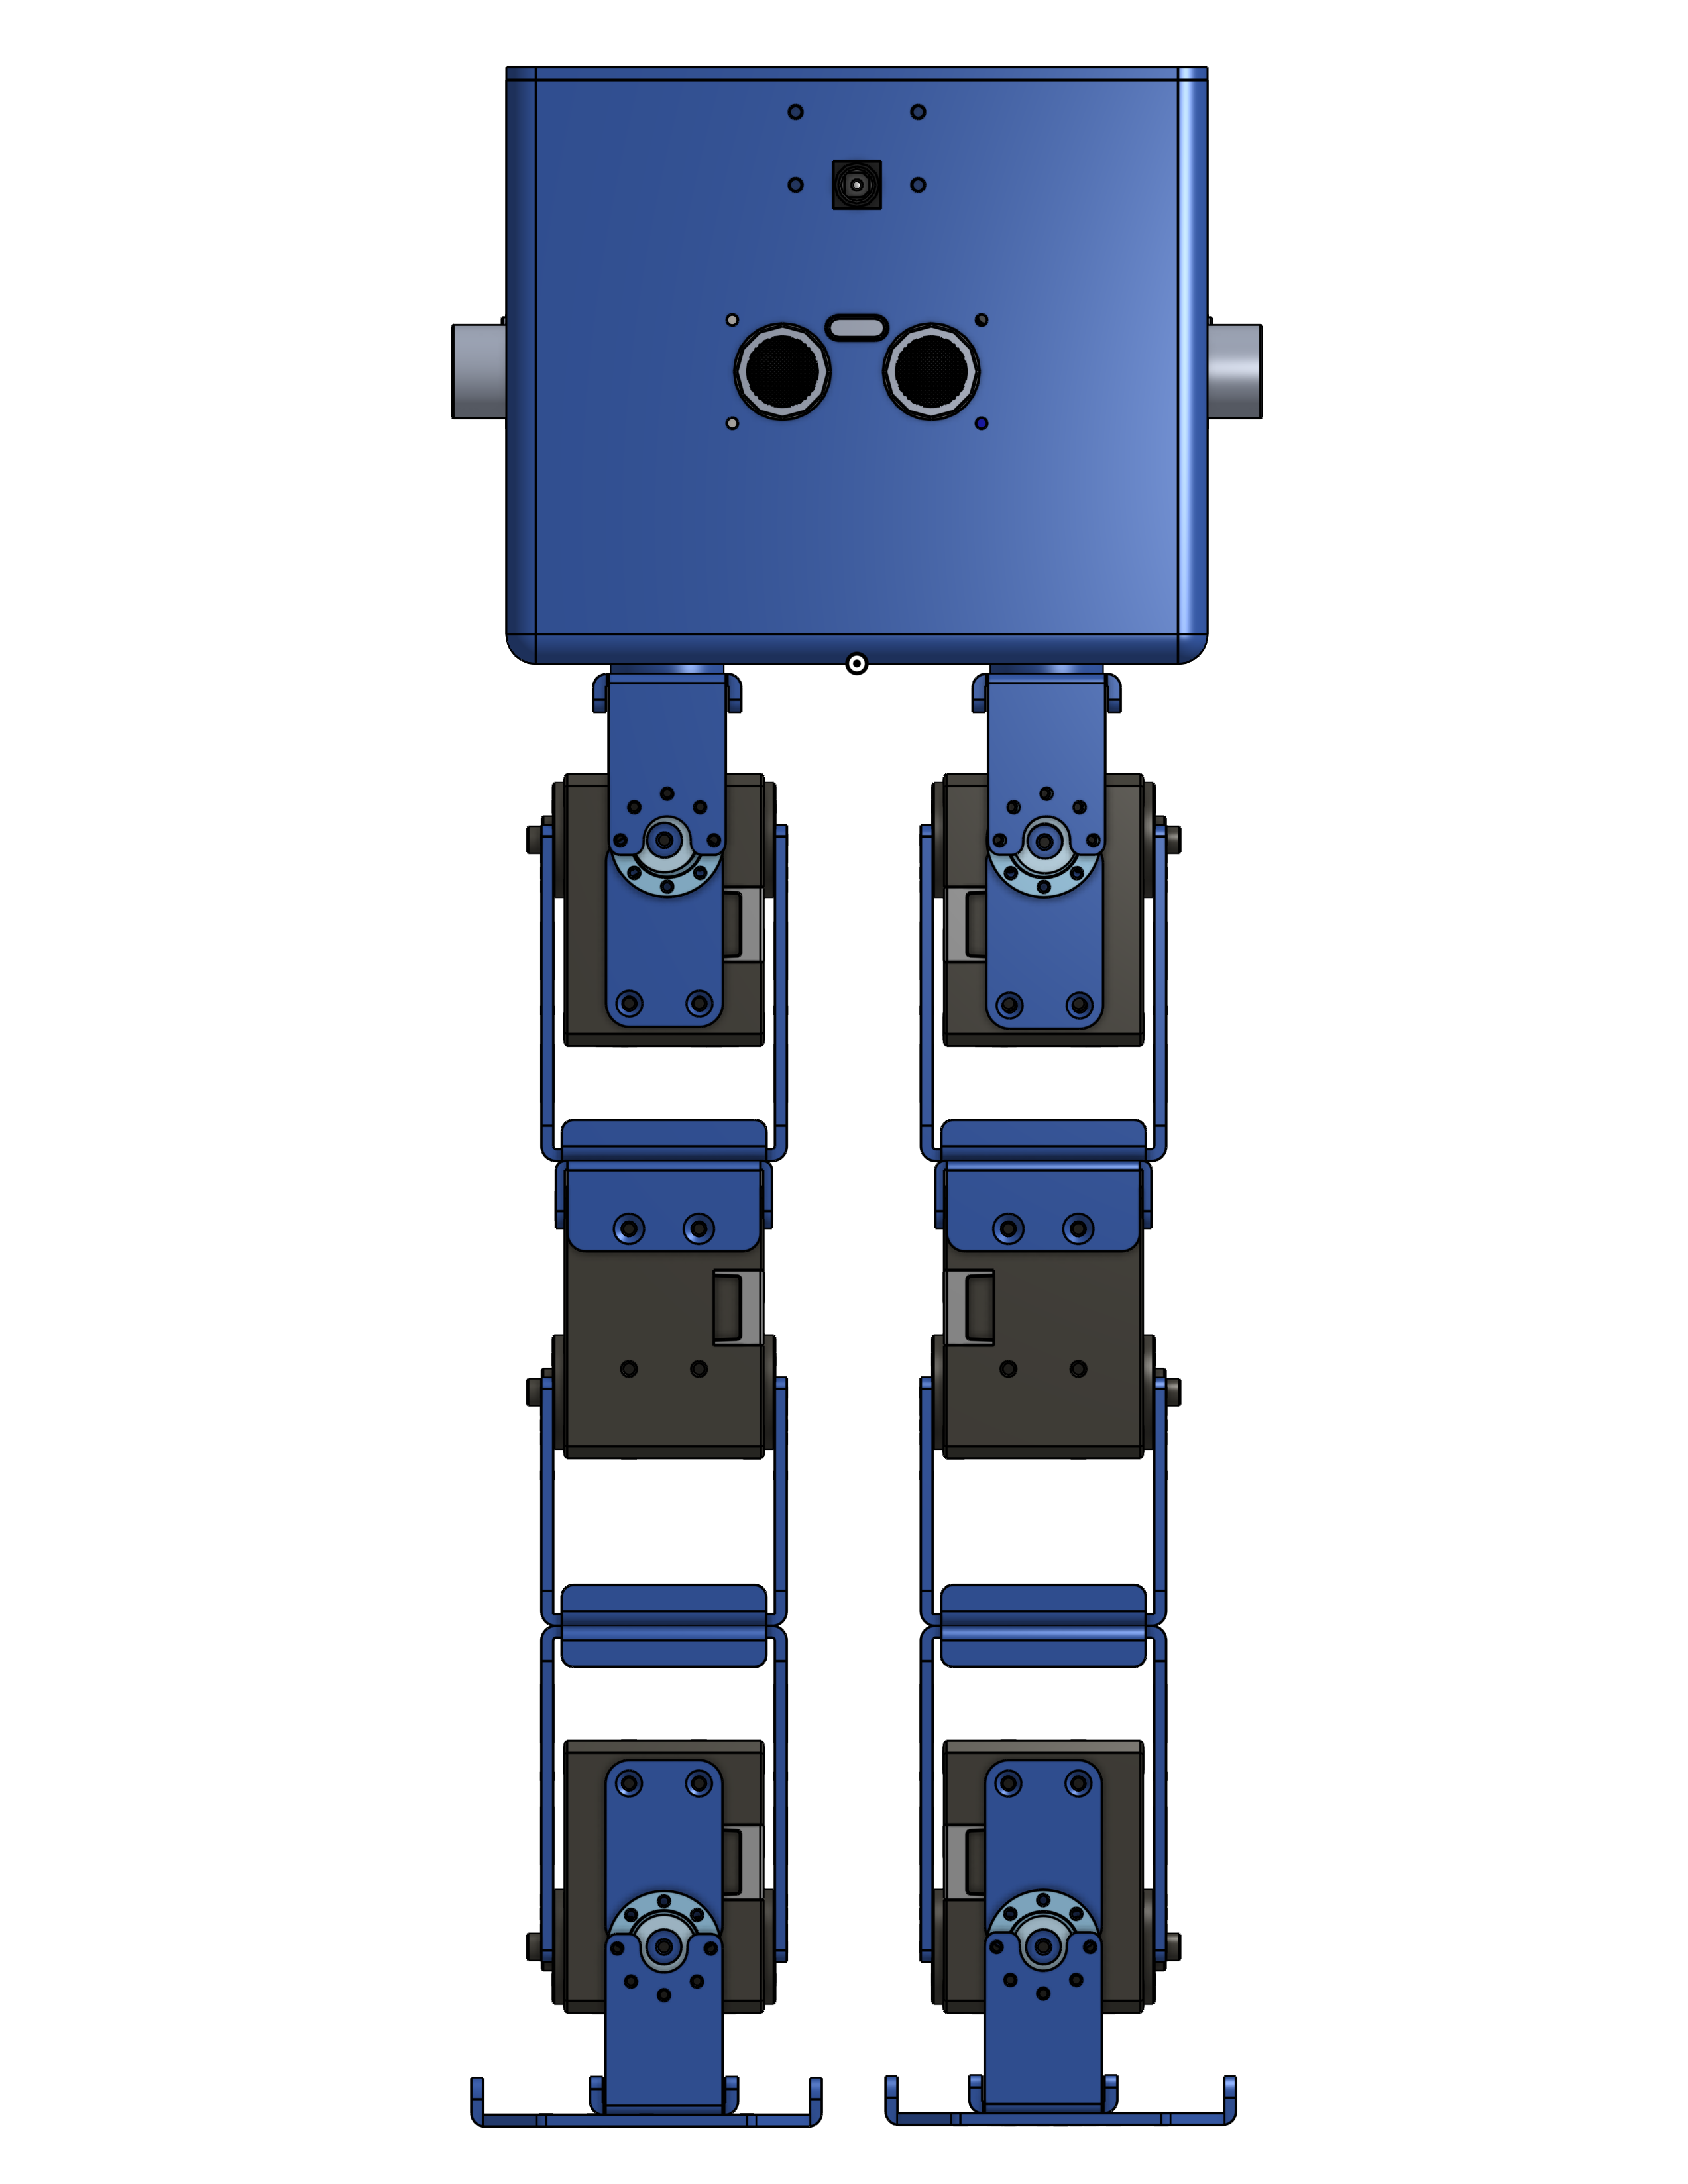
\includegraphics[width=\textwidth]{walker_3Dfrontal}

    \end{columns}
\end{frame}
%-


%*----------- SLIDE -------------------------------------------------------------
\begin{frame}[t]{Montagem do URDF} 
    \begin{columns}
        \column{.65\textwidth}
        \centering
        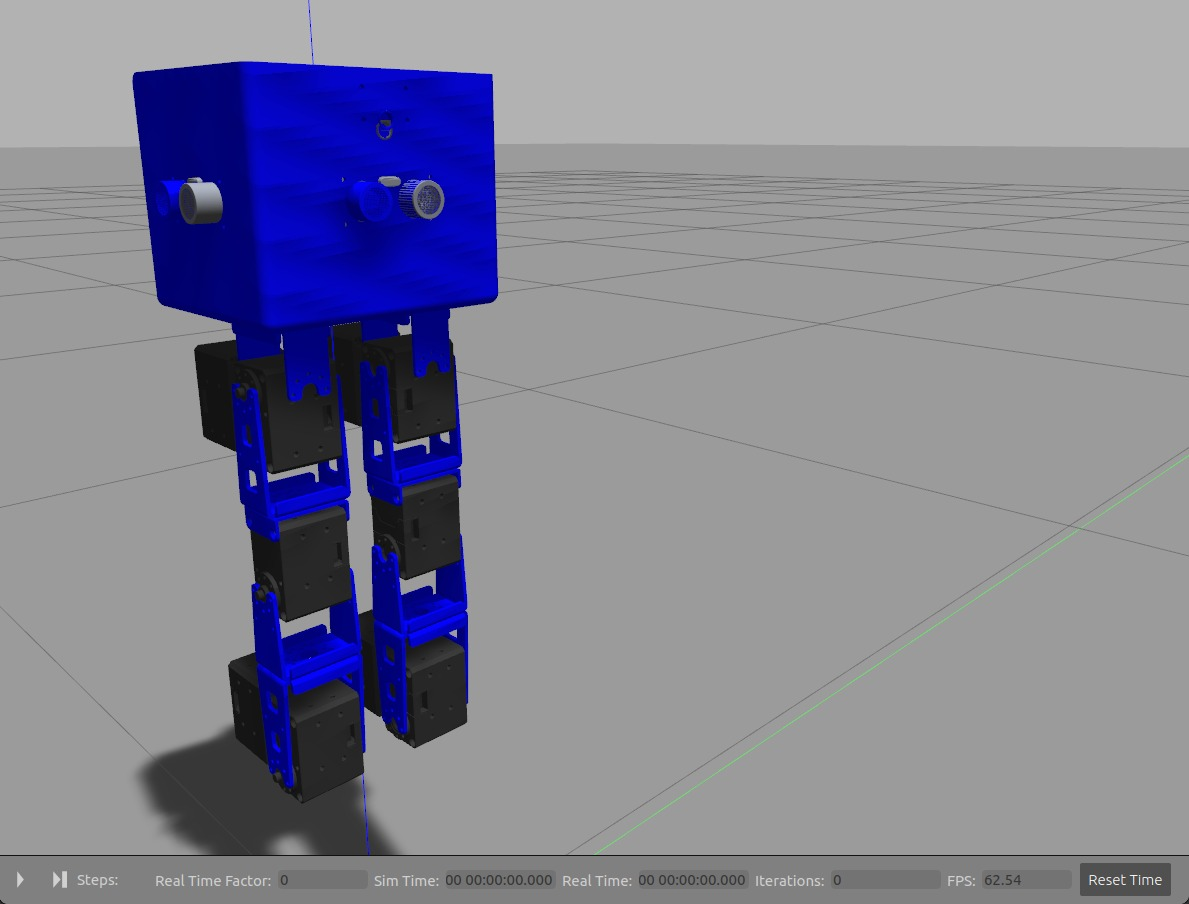
\includegraphics[width=.92\textwidth]{walker_urdf}

        \column{.35\textwidth}
        \textbf{Criação dos pacotes:}
        \begin{itemize}
            \item walker\_description
            \item walker\_gazebo
        \end{itemize}
        \vspace{.5cm}
        \textbf{URDF:}
        \begin{itemize}
            \item Criação e posicionamento dos links
            \item Adição dos plugins dos sensores
            \item Transmissão dos motores
        \end{itemize}
    \end{columns}
\end{frame}
%-

%*----------- SLIDE -------------------------------------------------------------
\begin{frame}[t]{Initial Design} 

    \centering
    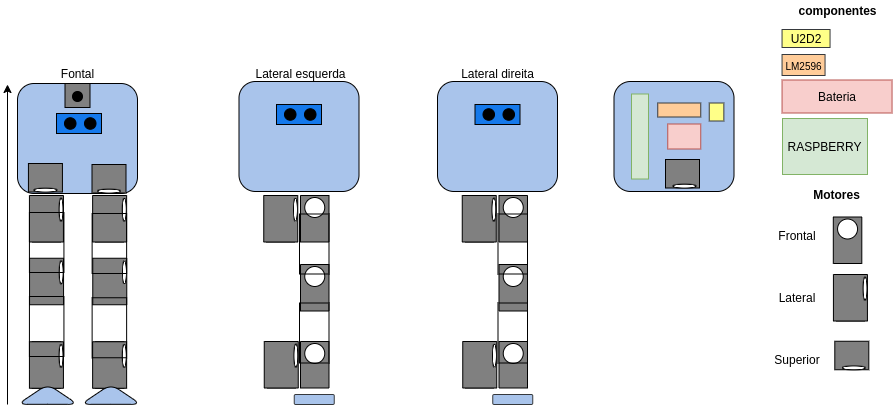
\includegraphics[width=.9\textwidth]{initial_design.png}

\end{frame}
%-

%*----------- SLIDE -------------------------------------------------------------
\begin{frame}[t]{Análise de riscos do projeto} 
    \begin{enumerate}
        \item Incompatibilidade da comunicação entre dynamixels e ROS Noetic
        \begin{enumerate}
            \item Adaptar os pacotes disponíveis para o ROS Melodic para o Noetic
        \end{enumerate}   
        \item Falta de informações sobre o mapa coletadas pelo sensor ultrassônico 
        \begin{enumerate}
            \item Incluir mais dois sensores, cada um na lateral do robô
            \item Substituir sensor ultrassônico por um LIDAR
        \end{enumerate}  
    \end{enumerate}
    
\end{frame}
%-
%-
%*----------- SLIDE-BACKUP ------------------------------------------------------
% \backupbegin
% %
% \begin{frame}{Backup}
%     Test
% %*----------- notes-------------------------------
% \note{Notes can help you to remember important information. Turn on the notes option.}
% \end{frame}
% %-
% \backupend
% %-
%*----------- QUESTIONS ---------------------------------------------------------
\begin{frame}[c,plain]
    \lastpage{
        \begin{center}   
            {\usebeamerfont{title} Questions?}\\[3ex] 
            %\hspace{1.5cm} 
            juliana.maria@fbter.org.br
        \end{center}
    }
    
    %*----------- notes---------------------------------
    \note[item]{Notes can help you to remember important information. Turn on the notes option.}
\end{frame}
%*-------------------------------------------------------------------------------
\end{document}